\documentclass[11pt,oneside]{book}
\usepackage[margin=1.5in]{geometry}
\renewcommand{\baselinestretch}{1.3}
\usepackage{graphicx}
\usepackage[square,numbers]{natbib}
\usepackage[italian]{babel}
% le immagini vanno tutte in images/
\graphicspath{{images/}}
\usepackage{amssymb}
\usepackage{amsthm}
\usepackage{graphics}
\usepackage{amsmath}
\usepackage{amstext}
\usepackage[nottoc]{tocbibind}
\usepackage{engrec}
\usepackage{microtype}
\usepackage{enumerate}
\usepackage{marginnote}
\usepackage{fancyhdr}
\usepackage{setspace}
\usepackage{bm}
\usepackage{float}
\usepackage[utf8x]{inputenc}
\usepackage{hyperref}
\usepackage{listings}
\pagestyle{plain}
\thispagestyle{empty}
\usepackage{minted}


\begin{document}
    \begin{titlepage}
            
        \noindent
        \begin{minipage}[t]{0.19\textwidth}
            \vspace{-4mm}{
\includegraphics[scale=1.15]{logo_unimib.png}}
        \end{minipage}
        \begin{minipage}[t]{0.81\textwidth}
        {
            \setstretch{1.42}
                {\textsc{Università degli Studi di Milano - Bicocca}} \\
                \textbf{Scuola di Scienze} \\
                \textbf{Dipartimento di Informatica, Sistemistica e Comunicazione} \\
                \textbf{Corso di laurea in Informatica} \\
                \par
        }
        \end{minipage}
            
    	\vspace{35mm}
            
    	\begin{center}
            {\Huge{
                    \setstretch{1.2}
                    \textbf{Detecting Fraud in Payment Services via Machine Learning}
                    \par
                }
            }
        \end{center}
            
        \vspace{35mm}
    
        \noindent
            {\large \textbf{Relatore:} Dr. Antonio Candelieri} \\

        \noindent
            {\large \textbf{Co-relatore:} Dr. Andrea Catacchio}
            
        \vspace{15mm}
    
        \begin{flushright}
            {\large \textbf{Relazione della prova finale di:}} \\
            \large{Artemisia  Sarteschi} \\
            \large{Matricola 829677} 
        \end{flushright}
            
        \vspace{11mm}
        \begin{center}
            {\large{\bf Anno Accademico 2019-2020}}
        \end{center}
    
        \restoregeometry
            
    \end{titlepage}
%\clearpage

\cleardoublepage
\thispagestyle{empty}
\vspace*{\stretch{1}}
\begin{flushright}
\itshape
\begin{tabular}{@{}l@{}}
Quando la strada non esiste, inventala! \\
\end{tabular}\\[3pt]
B. -P. \\


\end{flushright}
\vspace{\stretch{2}}
\cleardoublepage

\thispagestyle{empty}
\frontmatter
\tableofcontents
\mainmatter
\chapter{Introduzione}
Il riciclaggio di denaro è una particolare tipologia di frode molto frequente all'interno degli istituiti bancari, per questo motivo studiare tecniche e approcci che ne permettano l'individuazione e la conseguente segnalazione all'autorità è di fondamentale importanza.
Il progetto di stage si è focalizzato su questo tema, andando a studiare un approccio che attraverso l'analisi delle transazioni di una banca portasse all'individuazione di schemi e comportamenti fraudolenti tra i clienti.

Il comportamento di ogni cliente viene analizzato per andare ad individuare delle anomalie nel suo comportamento durante il tempo, ad esempio se le sue abitudini di spesa sono costanti o ha dei picchi anomali in determinati periodo di tempo non coincidenti con festività o periodi di tassazione. 
Inoltre, ognuno dei clienti non viene analizzato solo singolarmente ma bensì anche in relazione agli altri utenti presenti nella banca, stabilendo se il suo comportamento è anomalo e quindi va a discostarsi significativamente dagli altri oppure rimane coerente con la popolazione.

Per effettuare queste analisi l'approccio che viene proposto si basa su delle tecniche di Machine Learning supervisionato e non supervisionato, che combinate portano alla delineazione di comportamenti fraudolenti e alla conseguente segnalazione di clienti anomali. 

\chapter{L'identificazione automatica di schemi fraudolenti in transazioni bancarie}

\section{Definizione di transazioni fraudolente}

Nell'andare a definire una transazione fraudolenta partiamo dal definire cosa si intenda per frode. 
Essa è definibile come un comportamento o azione ingannevole progettata per fornire all'autore un guadagno scorretto o illegale oppure per negare un diritto a una vittima. 
L’autore della frode può essere un singolo individuo, ma anche più persone fino ad arrivare ad un intera azienda.

Le frodi implicano una falsa rappresentazione dei fatti, realizzata sia nascondendo intenzionalmente informazioni salienti, sia fornendo false dichiarazioni con lo scopo di ottenere qualcosa che non potrebbe essere ottenuto senza l’inganno. 
Esse possono verificarsi in ambito: finanziario, immobiliare, d’investimenti e assicurativo, includono varie tipologie come la frode con carte di credito, fiscale, telematica, finanziaria e in caso di bancarotta.

Fondamentalmente, l’individuo o l’azienda che commette una frode si avvale di asimmetrie nelle informazioni, in modo particolare sfrutta la necessità di impiegare una quantità di risorse molto elevata per la revisione e verifica delle informazioni che portano ad un disincentivo nella prevenzione della frode.

L'ambito su cui il progetto di stage si focalizza è sull'analisi di transazioni fraudolente svolte nell'ambito dell'antiriciclaggio che solitamente si realizzando con transazioni frequenti di piccole somme e/o grossi spostamenti di denaro in entrata ed in uscita con un saldo finale nullo.



\section{Il tema dell'antiriciclaggio}

Il riciclaggio (money laundering) viene legalmente definito come “un trasferimento di denaro ottenuto illegalmente tramite persone o conti legittimi cosicché la fonte originale non possa essere tracciata”\citep{teher}.
Questo denaro ottenuto illegalmente, definito ``denaro sporco",  viene quindi depositato in istituti finanziari e dal momento che sembrerà provenire da fonti legali non attirerà l’attenzione delle forze dell'ordine.

I profitti ottenuti attraverso questo processo vengono talvolta impiegati per finanziare crimini, includendo terrorismo, traffico di droga e vendita di armi illegali. 
La stima del profitto mondiale ottenuto tramite il riciclaggio di denaro in un anno è approssimatamene il 2-5\% del PIL globale (GDP) . %\citep{pil}.

Il riciclaggio si compone di tre stadi:

\begin{itemize}

\item \textbf{\textit{Collocamento}}: lo stadio più rischioso in cui ingenti somme di denaro sporco vengono spostate dalla sua fonte negli istituti finanziari, sia locali che esteri. 

\item \textbf{\textit{Stratificazione}}: l’obbiettivo di questo stadio è rendere difficile rilevare, scoprire e tracciare il denaro ``sporco". Si tratta di un processo molto sofisticato in cui vengono effettuate diverse spostamenti di denaro tramite bonifici tra conti, con nomi e paesi differenti, vari trasferimenti tra banche, depositi e prelievi con diverse somme di denaro e cambi di valuta. 

\item \textit{\textbf{Integrazione}}: l’ultimo e più semplice stadio tra i tre ed inoltre il più difficile da rilevare.
La difficoltà nel rilevamento è insita nella difficoltà nell'identificare un riciclatore senza documentazione che provi i due stadi precedenti.
Il denaro precedentemente ottenuto, ora legittimo perché proveniente da transazioni legali, viene ora impiegato per acquistare beni o per continuare a finanziare attività illegali.
\end{itemize}

Il termine \textit{antiriciclaggio} indica tutte le procedure, leggi, politiche, regolamenti e atti legislativi che impongono gli istituti finanziari per monitorare i loro clienti e per impedire il riciclaggio. Questo richiede inoltre alle istituzioni finanziare di segnalare qualsiasi reato finanziario che rilevano e bloccarlo. 


I sistemi antiriciclaggio (Anti-Money Laudering - AML) sono implementati dagli istituti finanziari come banche e da altri organismi che forniscono credito, in modo tale da combattere il fenomeno identificando scenari, potenziali attori e le transazioni coinvolte.


Questi sistemi software sono progettati per aiutare gli istituti finanziari a combattere il riciclaggio analizzando i dati che compongono i profili dei clienti identificando transazioni sospette e anomale, che includono ogni incremento di denaro improvviso o un ampio prelievo, ma anche piccole transazioni sono segnalate come sospette.

Tuttavia le tecniche di riciclaggio sono sempre più sofisticate e difficili da identificare perché cercano sempre più di annidarsi nel grande volume di dati e transazioni delle banche che creano un ambiente ideale per nascondere il denaro sporco. 

Le soluzioni devono quindi evolvere bilanciando accuratezza e tempo di processamento, durante il corso degli ultimi anni ci sono state moltissime soluzioni proposte che generalmente in una prima fase raccolgono e processano i dati, poi controllano e monitorano le transazioni e se una di queste è anomala la segnalano ad un analista che deciderà se segnalarla come fraudolenta.

Generalizzando possiamo vedere come i sistemi AML seguano uno schema composto da quattro layer \citep{han2020artificial}.

\begin{itemize}
\item \textit{Data Layer}: in cui i dati più rilevanti vengono raccolti e archiviati, includendo: sia quelli interni provenienti dall'istituto finanziario, sia quelli esterni provenienti da altre fonti come autorità, enti regolatori o da liste di controllo.
\item \textit{Screening and Monitoring Layer}: all'interno del quale le transazioni e i clienti vengono controllati, in modo quasi totalmente automatizzato, per cercare attività sospette e nel caso in cui fossero trovate si passa al layer successivo.
\item \textit{Alert and Event Layer}: nel caso in cui alcune transazioni fossero segnalate come anomale vengono passate in questo layer per un ulteriore verifica. Questo processo compara i dati della transazione segnalata con le informazioni sulle transazioni storiche e eventuali informazioni in possesso dell'istituto finanziario o di fonti esterne.
\item \textit{Operational Layer}: in cui un analista prende la decisione definitiva di bloccare o approvare la transazioni.
\end{itemize}

Questi layer sopracitati sono stati adottati come schema base anche nel progetto di stage in cui tramite analisi di diverse metriche descritte nei capitoli seguenti ed applicando algoritmi machine learning siamo riusciti a visualizzare persone potenzialmente fraudolente.
\chapter{Soluzioni data-driven per la ``fraud-detection'': lo stato dell'arte}



Tra le varie soluzioni che sono impiegate per rilevare le frodi nell'ambito del riciclaggio, durante il progetto di stage ci siamo focalizzati su quelle ``data-driven''. I dati sono stati utilizzati come base per le decisioni e le strategie impiegate, eliminando tutta la componente di considerazioni personali e osservazioni tipiche di altri approcci.

Per l'analisi di questi dati ci siamo basati su algoritmi di apprendimento automatico (Machine Learning-ML),  un sottoinsieme dell'intelligenza artificiale (Artificial Intelligence - AI) che rende i computer in grado di imparare in modo autonomo dall'esperienza senza essere esplicitamente programmati per farlo.
Durante il corso degli ultimi anni questi algoritmi sono stati largamente impiegati nell'antiriciclaggio perché fondamentali nella riduzione delle percentuali di falsi positivi e nell'individuazione tempestiva di transazioni sospette.

Le due principali famiglie di algoritmi di ML attualmente utilizzati sono gli algoritmi supervisionati e non supervisionati. La differenza tra questi due approcci viene definita dal modo in cui ciascun algoritmo apprende i dati per fare previsioni. 

Gli algoritmi di \textit{apprendimento supervisionato} (supervised machine learning) imparano da un dataset di addestramento passato dal supervisore, precedentemente etichettato e con un attributo target predefinito (output), contenente transazioni e schemi sia anomali che normali per andare a costruire il modello predittivo. Il dataset su cui viene fatto l'addestramento dell'algoritmo deve essere inoltre ben formato prima di applicare tecniche e algoritmi di machine learning. 
Questo approccio è adatto per quelle banche che che hanno un esperienza pregressa nel rilevare il  riciclaggio di denaro. 


Nel caso invece dell'\textit{apprendimento automatico senza supervisione} (unsupervised machine learning), gli algoritmi lavorano su insieme di dati privi di etichette, senza riferimenti noti, per cui non è stato definito un output specifico.
L'algoritmo lavora senza supervisione basandosi solamente sulle sulle informazioni latenti del dataset non etichettato e non necessita di un reale addestramento.
L'obiettivo di apprendimento senza supervisione è scoprire modelli nascosti, somiglianze, strutture nascoste e raggruppamenti di dati senza alcuna formazione preliminare. Questo approccio è adatto per le banche che non dispongono di metodi per esaminare i dati e non dispongono di conoscenza pregressa, ma anche per tutti gli istituti finanziari che vogliono cercare nuovi schemi e individuare un numero maggiore di frodi.

Sulla base dei risultati ottenuti dalle ricerche più recenti sulle soluzioni da adottare in campo AML si è visto come le attuali tecniche prestano particolare attenzione alla qualità del dataset e alla scelta dell'algoritmo di ML ottimale per i dati forniti.
In un primo momento, i dati grezzi ottenuti dalle istituzioni finanziarie vanno spesso a tradursi in volumi di dati estremamente grandi e sbilanciati, che alcuni studi recenti suggeriscono di gestire applicando tecniche supervisionate. 

Etichettando quando possibile come normale o sospetta una transazione sulla base degli esempi forniti, l'algoritmo crea un modello di apprendimento supervisionato per classificare i nuovi dati in diverse categorie.

Tuttavia, altri studi suggeriscono di applicare tecniche non supervisionate, che consistono in algoritmi che cercano di separare i dati in gruppi diversi senza basarsi su un insieme di dati precedentemente etichettati. Questi gruppi di oggetti, noti come cluster, presentano tra loro delle similarità, ma allo stesso tempo presentano caratteristiche differenti con oggetti appartenenti ad altri cluster.
Sebbene a volte la tecnica di apprendimento senza supervisione contenga anche un insieme di dati di addestramento, l'etichetta dei dati verrà omessa durante il processo di apprendimento e verrà utilizzato per la valutazione dopo aver generato i cluster. 
Questo approccio viene ripreso nei lavori proposti in \citep{le2010application, larik2011clustering}. Nel primo viene adottato un sistema di AML attraverso un particolare algoritmo non supervisionato chiamato K-means che attraverso la distanza tra cluster cerca di identificare gli utenti che compiono transazioni anomale. Nel secondo viene principalmente impiegata la deviazione tra i cluster per definire transazioni normali e anomale.

Nello studio condotto in \citep{omar2013machine} dove varie tecniche di ML vengono confrontate, emerge che le tecniche supervisionate siano più performanti delle non supervisionate, nel caso in cui il dataset non presenti tipologie di attacchi sconosciute. In caso contrario, gli algoritmi di ML non supervisionato sono più performanti, dal momento che non si basano su un insieme di dati su cui l'algoritmo è stato allenato, ma cercano di aggregare ed isolare tutte quelle transazioni che si discostano dal normale.

Poiché le operazioni finanziarie possono variare di volta in volta, vi è una costante necessità di nuovi metodi, tecniche e modelli che possano rilevare in anticipo nuovi schemi di riciclaggio ed allo stesso tempo monitorare quelli conosciuti. 

Per questo motivo, nel corso del progetto di stage abbiamo eseguito inizialmente dei test su un dataset sperimentale applicando un approccio supervisionato, ma ci siamo poi concentrati su un approccio non supervisionato una volta passati ai dati reali.






\chapter{L'approccio proposto}
\section{Identificazione automatica di clienti con comportamenti atipici}

L’identificazione dei clienti che stanno effettuando delle transazioni fraudolente è il tema centrale dell'antiriciclaggio. Al fine di individuare queste persone, durante il progetto di stage è stato deciso di identificarli attraverso un approccio basato sull'individuazione di comportamenti anomali nelle loro transazioni.
Il fine del progetto è quello di sviluppare un algoritmo non supervisionato che identifichi, in modo automatico, tutti quei soggetti che hanno un comportamento anomalo rispetto a tutti gli altri appartenenti alla stessa banca.

Per l'identificazione di tutti quei comportamenti da segnalare come anomali l'approccio è stato basato sul clustering, ovvero sul raggruppare in cluster soggetti con
comportamenti simili tramite l'osservazione delle loro transazioni nell'arco
temporale di un mese, tutti i clienti che non andavano ad inserirsi in uno dei cluster
venivano successivamente posti sotto osservazione.

Tuttavia un solo discostamento dal cluster non è una motivazione sufficiente per segnalare un soggetto come fraudolento, tale movimento può essere avvenuto a causa di particolari festività oppure a causa di un evento imprevisto nella vita del cliente.
Per questo motivo ogni cliente viene monitorato per vari mesi e se questo comportamento si ripete per un numero di volte fissato viene deciso di segnalarlo.

Il discostarsi da un cluster, quindi avere un comportamento differente rispetto a tutti gli altri clienti della banca non è l'unico comportamento che viene tenuto sotto controllo nel monitoraggio di possibili comportamenti fraudolenti.
Infatti, un altro segnale di riciclaggio, è lo spostamento frequente da un cluster ad un altro di un cliente, infatti un comportamento normale di un cliente dovrebbe essere quello di muoversi all'interno del cluster con piccole variazioni dovute a normali eventi esterni.

La finalità del progetto è stato quindi quello di creare un algoritmo che analizzasse le transazioni di ogni cliente all'interno di un singolo mese, quindi su un intervallo di trenta giorni, analizzando attraverso differenti variabili descrittive il loro comportamento soffermandoci principalmente sul loro comportamento rispetto ai cluster: variavano spesso cluster o diventavano punti isolati senza mai essere riassorbiti.
Quando questi comportamenti atipici si ripetono più volte nel tempo parte quindi la segnalazione.



\section{Le principali variabili descrittive}

Per identificare i comportamenti fraudolenti dei clienti, vengono selezionate diverse variabili descrittive che incrociate fra loro producano evidenze di ciò che è oggetto del progetto:
\begin{itemize}
\item Numero di operazioni totali effettuate da una singola persona in un mese
\item Numero di operazioni totali di incremento del conto corrente
\item Numero di operazioni totali di decremento del conto corrente
\item Numero di giorni in cui sono state effettuate operazioni di incremento del conto corrente
\item Numero di giorni in cui sono state effettuate operazioni di decremento del conto corrente
\item Numero di giorni in cui sono state effettuate operazioni sia di incremento che di decremento del conto corrente
\item Numero totale di giorni in cui sono state effettuate operazioni di qualsiasi genere
\item Importo totale movimentato da operazioni di qualsiasi tipi in un mese
\item Importo totale movimentato in operazioni di incremento in un mese
\item Importo totale movimentato in operazioni di decremento in un mese
\item Transazione minima 
\item Transazione massima 
\item Saldo medio di ogni cliente 
\item Saldo minimo di ogni cliente 
\item Saldo massimo di ogni cliente 
\item Saldo finale di ogni cliente 
\end{itemize}


\section{Clustering mensile e anomalie ``statiche"}
Tramite l'ausilio delle variabili precedentemente introdotte sono state monitorate delle configurazioni di transazioni che potevano risultare appartenere ad una  possibile frode nel ambito del riciclaggio di denaro.
L'approccio che è stato deciso di proporre si compone di una parte \textit{statica}, ovvero di un analisi focalizzata su ciò che avviene in un determinato lasso di tempo senza compararlo con ciò che è avvenuto prima o dopo, ed è quella che andiamo ad analizzare in questo paragrafo, ed una \textit{dinamica} che analizzeremo nel paragrafo successivo.

Nel nostro caso il periodo di tempo considerato è stato un mese, con cui si intende un mese di calendario (es. Febbraio, Marzo...) e non un periodo di 30 giorni, questo perché lavorando con una banca è di più facile estrazione un mese con questa accezione. In aggiunta, nel momento in cui una frode dovesse essere segnalata sarà più facile il recupero delle transazioni in un mese predefinito, rispetto ad periodo di tempo da noi scelto arbitrariamente.

Effettuiamo quindi un clustering mensile, presi tutti i clienti che in quel mese hanno effettuato operazioni, tramite un clustering di tipo gerarchico sono stati formati dei cluster dell'intera popolazione di clienti della banca. 

L'analisi è stata condotta producendo anche degli scatterplot per poter analizzare in modo visivo la composizione dei cluster e renderne la comprensione più semplice per gli operatori che in seguito andranno a visionare gli eventuali clienti segnalati come possibili fraudolenti.
Questa facilità di visualizzazione è data dalla colorazione differente che ogni cluster possiede rendendo più semplice individuare l'appartenenza di un componente ad un determinato cluster.

\begin{figure}[H]
    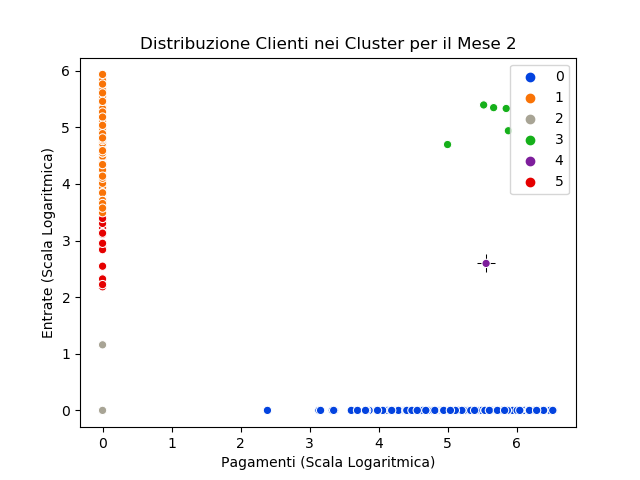
\includegraphics[width=0.9\textwidth]{M2.png}
    \centering
    \caption{Scatterplot di esempio}
    \label{fig:esScatter}
\end{figure}

Quando dalla scomposizione degli utenti in cluster viene rilevato che un utente forma un cluster singolo, ovvero in cui l’unico componente è lui e non sono presenti altri clienti, viene segnalato come anomalo sollevando un \textit{alert} su di lui.

Nel momento in cui un utente è l’unico componente di un cluster significa che ha avuto un comportamento anomalo rispetto a tutti gli altri clienti della banca in quel mese, viene quindi segnalato anche nel caso in cui sia la prima volta che questo accade. La segnalazione non equivale ad affermare che quella persona stia effettuando una frode, ma piuttosto a porla sotto osservazione per andare ad analizzare se quel comportamento è un avvenimento isolato oppure è parte di uno schema di riciclaggio di denaro.
Nel caso in cui dovesse risultare da un analisi longitudinale che questa persona è risultata anomala per vari mesi allora il livello di attenzione a cui è sottoposto incrementerebbe e si aggiungerebbe il flag di possibile persona fraudolenta.

Durante l'analisi è stato deciso di non soffermarsi solo sulla particolarità di formare cluster singoli ed essere quindi etichettati come un anomalia, ma è stato deciso di approfondire l'analisi di questa particolarità andando ad individuare delle \textit{regole} ovvero delle spiegazioni delle anomalie che questi utenti hanno prodotto attraverso i loro movimenti.

Queste regole, una volta che questi utenti sono riconosciuti come realmente fraudolenti, possono essere impiegate in AML come schema conosciuto di riciclaggio e riconoscere in minor tempo future frodi e prevenirle.

Per definire le \textit{regole} che caratterizzano un cliente, o più clienti, con comportamento anomalo all'interno di un mese è stato, come prima cosa, identificato il numero di cluster formati dai clienti in quel mese e il numero di componenti di ognuno. Il numero di cluster si è reso necessario perché il setting sperimentale (basato su dati reali) su cui è stato testato il nostro approccio è molto esiguo e in alcuni mesi comprendeva un solo utente oppure un solo cluster a cui appartenevano tutti i clienti. Un altra casistica che poteva accadere, a causa della quale il mese doveva essere scartato, era la presenza di più cluster ma tutti con un numero di utenti maggiore di uno.
Durante questa fase vengono inoltre creati degli scatterplot per vedere anche in modo grafico i cluster formati dai clienti in quel mese come in figura \ref{fig:esScatter}.

Nel momento in cui sono stati identificati i mesi in cui era presente un cluster formato da una sola persona, solitamente molto distante anche graficamente da tutti gli altri, ci si è andati a concentrare su ogni singolo mese andando a segnalare il cliente potenzialmente fraudolento.
Il dataset iniziale in cui comparivano tutte le transazioni aggregate e riassunte di quel mese è stato quindi arricchito di una colonna \textit{Fraud} che valeva 0 nel caso in cui quel utente non fosse segnalato come fraudolento e 1 nel caso in cui avesse formato un cluster singolo e quindi fosse da tenere sotto osservazione.
Questo dataset così composto è stato dato in input ad un \textit{Decision Tree Classifier }per andare ad estrarre le regole, intese come spiegazione dell'anomalia riscontrata, per il particolare cliente. 

Queste regole così estratte esprimono il comportamento del cliente e sono facilmente riconducibili al posizionamento dei punti sullo scatterplot (ognuno corrispondete ad un cliente) che vengono creati durante la fase di clustering, i risultati ottenuti da queste verranno discussi nei capitoli successivi. 

\section{Analisi longitudinale dei clusters e anomalie ``dinamiche"}

L’approccio che è stato deciso di proporre per l’identificazione di persone che attuano schemi di riciclaggio si compone di una parte \textit{statica}, descritta nel paragrafo precedente e una parte \textit{dinamica} che trattiamo in questo paragrafo.

Un anomalia \textit{dinamica} è un anomalia che viene identificata comparando tra loro i dati e le analisi relative a più mesi, possiamo associarla ad un cliente che presenta varie anomalie statiche nei mesi dell'orizzonte temporale considerato oppure ad un cliente che non è mai risultato anomalo ma ha effettuato un salto di cluster nell'ultimo mese.

L’analisi delle anomalie statiche di un mese produce come risultato una tabella in cui ogni identificativo (ID) di ogni utente è associato al cluster in cui si è trovato in quel mese ed eventualmente se è risultato anomalo. Partendo dalle tabelle così ottenute per tutto l’orizzonte temporale considerato andiamo a delineare le anomalie dinamiche. I dati contenuti in queste permettono di individuare se questo utente è stato già anomalo precedentemente nel periodo temporale considerato e quante volte lo è stato. Il numero di volte che questo è accaduto determina l’innalzare il livello di allerta di possibile comportamento fraudolento per quel utente, la \textit{regola statica} che viene fornita come spiegazione del comportamento sarà quella prodotta nell'ultimo mese in cui l'utente è stato anomalo.

Tuttavia, se l’utente non è mai risultato anomalo nel periodo considerato ma \textit{salta} ovvero cambia cluster vi sono delle considerazioni differenti da fare.

Le possibili motivazione alla base del cambio di cluster di un utente possono essere molteplici, una fra tutte il cambio di abitudini e quindi di profilo dell'utente. Lo spostamento frequente fra i cluster potrebbe comunque essere un segnale di comportamento fraudolento e necessita di segnalazione. 

Bisogna però tenere in considerazione la possibilità che i cluster si modifichino durante i mesi, unendosi o dividendosi in modo spontaneo, in questo caso non si tratterebbe di un vero e proprio salto, per questo motivo andiamo a considerare le sotto popolazioni all'interno di un cluster per mantenere una consistenza dei cluster tra i mesi.
Preso il cluster al mese precedente a quello considerato si va ad analizzare la composizione di esso e allo stesso modo si verifica la composizione del cluster a cui appartiene l’utente nel mese considerato, per questo motivo è di fondamentale importanza tenere traccia dei cluster a cui sono appartenuti i clienti in ogni mese.

Se nel cluster è presente una sotto popolazione del cluster del mese precedente allora l'utente non ha effettuato un salto di cluster, ma bensì si è mosso in maniera coerente rispetto alla sua sotto popolazione, non va quindi a rappresentare un anomalia.

Nel caso in cui il cluster del mese considerato non contenga nessun utente già presente nel cluster di cui faceva parte il cliente nel mese precedente, siamo di fronte ad un salto di cluster anomalo e come tale viene segnalato tramite un alert, se questo comportamento dovesse reiterarsi nel tempo è un segnale di possibile frode e il livello di attenzione su quel utente andrebbe ad incrementare.
Consideriamo anomalo quando è un solo cliente a saltare, quando invece sono almeno due il cambio di cluster potrebbe essere dovuto a motivi fiscali o legislativi e nel nostro caso non lo consideriamo anomalo.

Partendo quindi dalle anomalie statiche di ogni cliente e dalle regole che le descrivono, si segnalano nei mesi precedenti i clienti che sono risultati anomali tramite: il numero di mesi della finestra temporale in cui è stato sollevato un alert oppure dalla percentuale di segnalazioni rispetto al totale di transazioni di un utente.

Tutti questi dati raccolti vengono raccolti in una tabella riassuntiva finale che contiene: ogni utente con il proprio identificativo (ID), la motivazione ovvero la regola che abbiamo estratto in precedenza che spiega l'anomalia e il periodo temporale in cui sono stati rilevati come fraudolenti. L’operatore a cui questi dati sono destinati andrà quindi a valutare le transazioni del utente o degli utenti segnalati per capire se effettivamente siamo nel caso di transazioni finalizzate al riciclaggio di denaro oppure a movimenti legittimi. 



\section{Progettazione del prototipo, ambiente software e librerie utilizzati}

Durante il progetto di stage è stato sviluppato un prototipo come conclusione e sintesi dell'approccio \textit{statico} proposto e per permettere una più facile interpretazione per gli operatori finali. Il prototipo (chiamato in seguito anche \textit{demo}) prende in input i dataset relativi al periodo temporale di cui si vuole analizzare la scomposizione in cluster ed eventualmente, se presente, sottolineare una possibile anomalia statica. 
Per ogni mese del periodo temporale viene eseguito il clustering gerarchico e individuati i cluster ed il relativo numero di componenti, nel caso in cui all'interno del mese fossero presenti degli utenti con comportamento anomalo associabile ad un anomalia statica vengono evidenziati, come si può vedere nell'immagine \ref{fig:mese1}. Inoltre tramite dei barplot viene esplicitato la numerosità dei clienti fraudolenti in quel mese.

\begin{figure}[H]
    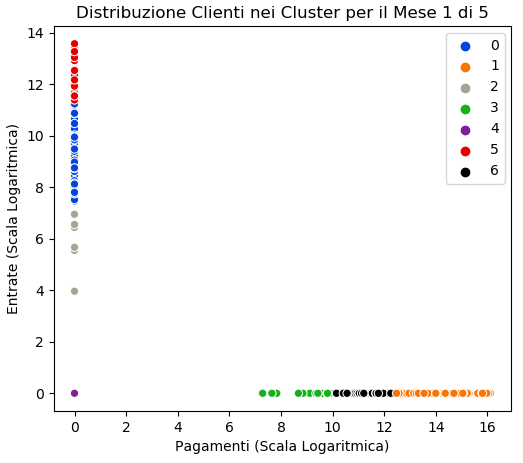
\includegraphics[width=0.8\textwidth]{Clustering_Mese_1.png}
    \centering
    \caption{Mese privo di clienti anomali}
    \label{fig:mese1}
\end{figure}
\begin{figure}[H]
    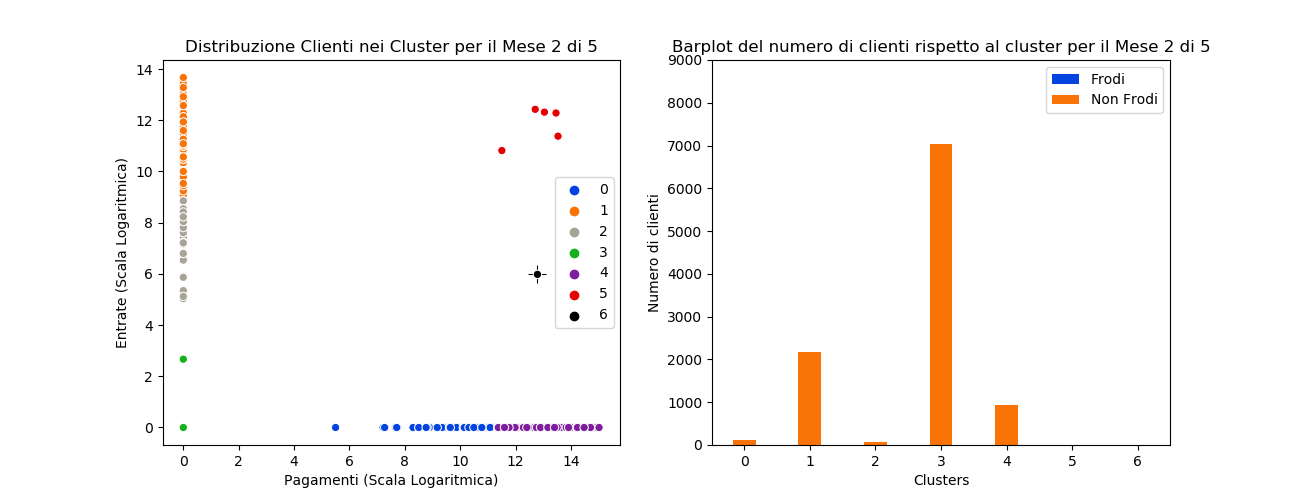
\includegraphics[width=1\textwidth]{Clustering_Mese_2.png}
    \centering
    \caption{Mese con un cliente anomalo}
\end{figure}


La demo è stata sviluppata in \textit{Python}, essendo il linguaggio utilizzato durante lo studio dell'approccio precedentemente descritto e la pre-elaborazione dei dati. \\ La piccola demo risultate è stata fornita come eseguibile al cliente per dare un primo sguardo su ciò che il progetto di stage arriverà ad essere. 


Per lo sviluppo della demo abbiamo impiegato le seguenti librerie:
\begin{itemize}
\item \textbf{Sklearn}\footnote{\url{https://scikit-learn.org/stable/index.html} in particolare Agglomerative Clustering } che fornisce supporto per molteplici algoritmi di machine learning, supervisionato e non supervisionato. 
\item \textbf{Seaborn}\footnote{\url{https://seaborn.pydata.org}}  per costruire grafici statistici in Python in particolare per la realizzazione di scatterplot e bar plot.
\end{itemize}


 %Nella nostra demo abbiamo utilizzato \textit{AgglomerativeClustering} per andare a creare i cluster mensili fondamentali per l'analisi delle anomalie statiche.

\chapter{Setting sperimentale}
\section{Open Data: una challenge Kaggle su fraud detection}


Durante il progetto di stage, in una prima fase di progettazione dell’approccio, è stato impiegato come dataset sperimentale un dataset di Kaggle chiamato \textit{Synthetic Financial Datasets For Fraud Detection} \citep{challenge}.
Questo dataset è stato impiegato dai vari utenti di Kaggle come base per analisi esplorative e addestramento di vari algoritmi di Machine Learning supervisionato. Poiché, durante il  progetto risultava necessario utilizzare tali algoritmi, è stato deciso di utilizzarlo per comprendere quale algoritmo fosse maggiormente performante nell'andare ad identificare le relazioni che intercorrono tra le frodi.

Inoltre, questo dataset è stato impiegato per lo sviluppo e la verifica della metodologia che  implementata per l'individuazione di anomalie statiche e dinamiche, conoscendo approfonditamente la composizione di questo dataset è stato possibile avere un riscontro immediato della validità dei risultati ottenuti.

Il dataset è formato da undici colonne (Tabella \ref{tab:primo}) per un totale di circa sei milioni di istanze ed ognuna di queste corrisponde ad una transazione, non si tratta però del dataset originale ma bensì di un quarto di esso che è stato estratto per essere messo a disposizione degli utenti Kaggle. \\




\noindent All'interno del dataset troviamo tre colonne i cui dati sono di tipo \textit{string} che contengono: 
\begin{itemize}
\item \textit{type}: tipologia di transazione
\item \textit{nameOrig}: cliente che ha eseguito la transazione
\item \textit{nameDest}: cliente che ha ricevuto la transazione
\end{itemize}

\noindent Inoltre, abbiamo cinque colonne di tipo \textit{decimale} che hanno al loro interno:

\begin{itemize}

\item \textit{amount}: importo della transazione nella valuta locale
\item \textit{oldbalanceOrg}: saldo iniziale prima che il cliente esegua la transazione 
\item \textit{newbalanceOrig}: saldo finale dopo che il cliente ha eseguito la transazione 
\item \textit{oldbalanceDest}: saldo iniziale prima che il cliente riceva la transazione 
\item \textit{newbalanceDest}: saldo iniziale finale dopo che il cliente ha ricevuto la transazione 

\end{itemize}

\noindent Infine, troviamo tre colonne di tipo \textit{intero}:

\begin{itemize}
\item \textit{step}: unità di tempo del mondo reale, in questo caso uno ``\textit{step}" corrisponde ad un'ora
\item \textit{isFraud}: transazioni che sono fraudolente (1) o non fraudolente (0)
\item \textit{isFlaggedFraud}: segnala i tentativi illegali di trasferire più di 200.000 unità in una singola transazione.\\

\end{itemize}

\begin{table}[H] %ht
\centering
\begin{tabular}{|c|c|c|c|c|c|} \hline
step & type & amount & nameOrig & oldbalanceOrg & newbalanceOrig \\ \hline
  ... & ...  & ... & ...  & ... & ... \\ \hline
\end{tabular}
\label{tab:primo}
\end{table}

\begin{table}[H] %ht
\centering
\begin{tabular}{|c|c|c|c|c|} \hline
nameDest & oldbalanceDest & newbalanceDest & isFraud & isFlaggedFraud \\ \hline
... & ... & ... & ... & ... \\ \hline
\end{tabular}
\caption{Colonne del dataset}
\label{tab:secondo}
\end{table}

Durante la preparazione del dato, dopo aver analizzato più a fondo il dataset, è stato deciso di eliminare la colonna \textit{isFlaggedFraud} che risulta essere non significativa per l'analisi che andremo a condurre. Inoltre, è stato scelto di memorizzare separatamente la colonna \textit{isFraud} per allenare successivamente gli algoritmi supervisionati, ed abbiamo infine rinominato alcune colonne per avere dei nomi più significativi.

Nell'analizzare il dataset è stato riscontrato come fossero presenti diversi casi in cui il saldo iniziale e finale rimanesse nullo, a fronte di una transazione con importo diverso da zero, sono state quindi segnalate queste anomalie con dei valori che l'algoritmo avrebbe facilmente riconosciuto come anomali. Oltre a ciò, è stata inserita una colonna contenente eventuali errori nel saldo.


Dal confronto con il cliente è risultato che sarebbe stato più utile avere come voci del dataset gli utenti e non le singole transazioni, sono stati quindi estratti i singoli utenti e create delle nuove colonne (Tabella \ref{tab:new}) che aggregassero le tipologie di transazioni a seconda del tipo. Queste nuove colonne rendono più chiaro le regole che verranno prodotte con \textit{Decison Tree}, perché si concentrano sulla tipologia di transazione e possiedono già al loro interno l'importo di essa. 



\begin{table}[H] %ht
\centering
\begin{tabular}{|c|c|c|c|c|c|c|} \hline
User ID & Entrate & Bonifici & Debit & Ricariche & Pagamenti & Estero
 \\ \hline
... & ... & ... & ... & ...& ... & ... \\ \hline
\end{tabular}
\caption{Colonne del nuovo dataset basato sulla challenge}
\label{tab:new}
\end{table}


\section{Un piccolo dataset reale}

Al termine dello sviluppo descritto nel capitolo precedente, l'approccio è stato testato su un piccolo dataset reale fornito dal cliente. 
All'interno di questo si trovano tutte le transazioni, con gli attributi più frequenti nei database delle banche (Tabella \ref{tab:reale}), di un ristretto gruppo di utenti nell'arco temporale di un anno.


Ispezionando il dataset per comprendere meglio i dati in esso contenuti è stato possibile rilevare come alcuni attributi non fossero rilevanti, in particolare: 
\textit{Descrizione Aggiuntiva} che sarebbe servito solo ad un operatore nel caso avesse avuto il compito di indagare sulle transazioni, \textit{Evidenza} il cui significato non ci era stato reso noto e \textit{Data} perché riporta la data contabile rispetto e non quella di esecuzione.\\


\begin{table}[H] %ht
\centering
\begin{tabular}{|c|c|c|c|c|c|c|c|c|} \hline
ID Transazione & ID Utente & Data & Descrizione & Valuta 
 \\ \hline
... & ... & ... & ... & ...\\ \hline
\end{tabular}
\label{tab:reale}
\end{table}
\begin{table}[H] %ht
\centering
\begin{tabular}{|c|c|c|c|c|c|c|c|c|} \hline
Evidenza & Importo & Saldo & Descrizione Aggiuntiva
 \\ \hline
... & ... & ... & ...  \\ \hline
\end{tabular}
\caption{Attributi completi del dataset reale}
\label{tab:reale}
\end{table}

Durante l'elaborazione dei dataset sono state estratte tutte le tipologie di transazione dalla colonna \textit{Descrizione} e rendendole degli attributi per rendere possibile conoscere chiaramente come i movimenti potenzialmente fraudolenti, di cui otteniamo le regole, sono stati effettuati.

Avendo inoltre la possibilità di conoscere precisamente la data della transazione è stato deciso di inserire dei nuovi attributi legati al numero di operazioni giornaliere per tipologia e importi movimentati, al fine di rendere più elaborate possibili le regole. Gli attributi inseriti sono i seguenti:

\begin{itemize}
\item \textit{Num\textunderscore Op\textunderscore Tot}: Numero di operazioni totali effettuate da una singola persona in un mese
\item \textit{Op\textunderscore In}: Numero di operazioni totali di incremento del conto corrente \textunderscore
\item \textit{Op\textunderscore Out}: Numero di operazioni totali di decremento del conto corrente
\item \textit{Num\textunderscore Giorni\textunderscore In}: Numero di giorni in cui sono state effettuate operazioni di incremento del conto corrente
\item \textit{Num\textunderscore Giorni\textunderscore Out}: Numero di giorni in cui sono state effettuate operazioni di decremento del conto corrente
\item \textit{Num\textunderscore Giorni\textunderscore In \textunderscore Out}: Numero di giorni in cui sono state effettuate operazioni sia di incremento che di decremento del conto corrente
\item \textit{Num\textunderscore Giorni\textunderscore Op}: Numero totale di giorni in cui sono state effettuate operazioni di qualsiasi genere
\item \textit{Amount\textunderscore Movim\textunderscore Tot}: Importo totale movimentato da operazioni di qualsiasi tipo in un mese
\item \textit{Amount\textunderscore Tot\textunderscore  In}: Importo totale movimentato in operazioni di incremento in un mese
\item \textit{Amount\textunderscore Tot\textunderscore  Out}: Importo totale movimentato in operazioni di decremento in un mese
\item \textit{Min\textunderscore Transaction}: Transazione minima (in valore assoluto)
\item \textit{Max\textunderscore Transaction}: Transazione massima (in valore assoluto)
\item \textit{Media\textunderscore Amount}: Saldo medio di ogni cliente
\item \textit{Min\textunderscore Amount}: Saldo minimo di ogni cliente 
\item \textit{Max\textunderscore Amount}: Saldo massimo di ogni cliente
\item \textit{Amount\textunderscore Finale}: Saldo finale di ogni cliente 
\end{itemize}

\noindent Le colonne finali del dataset considerato risultano essere le seguenti (Tabella \ref{tab:ti}).

\begin{table}[H] %ht
\centering
\begin{tabular}{|c|c|c|c|c|c|c|c|c|c|} \hline
ID\textunderscore Utente & Num\textunderscore Op\textunderscore Tot & Op\textunderscore In & Op\textunderscore Out & Num\textunderscore Giorni\textunderscore In & Num\textunderscore Giorni\textunderscore Out\\ \hline
... & ... & ... & ... & ...& ...\\ \hline
\end{tabular}
\end{table}
\begin{table}[H] %ht
\centering
\begin{tabular}{|c|c|c|c|} \hline
Num\textunderscore Giorni\textunderscore Out & Num\textunderscore Giorni\textunderscore In \textunderscore Out & Num\textunderscore Giorni\textunderscore Op & Amount\textunderscore Movim\textunderscore Tot \\ \hline
... & ... & ... & ...  \\ \hline
\end{tabular}
\end{table}

\begin{table}[H] %ht
\centering
\begin{tabular}{|c|c|c|c|} \hline
Amount\textunderscore Tot\textunderscore  In & Amount\textunderscore Tot\textunderscore Out & Min\textunderscore Transaction & Max\textunderscore Transaction \\ \hline
... & ... & ... & ...   \\ \hline
\end{tabular}
\end{table}

\begin{table}[H] %ht
\centering
\begin{tabular}{|c|c|c|c|} \hline
Media\textunderscore Amount & Min\textunderscore Amount & Max\textunderscore Amount & Amount\textunderscore Finale \\ \hline
... & ... & ... & ...  \\ \hline
\end{tabular}
\caption{Attributi completi del dataset reale dopo l'elaborazione}
\label{tab:ti}
\end{table}


\chapter{Risultati}
\section{Risultati su challenge Kaggle}
L'approccio proposto negli scorsi capitoli per l'identificazione delle anomalie statiche e dinamiche ha prodotto diversi risultati che andiamo a riportare in questo capitolo, in particolare questo paragrafo è incentrato sul setting sperimentale fornito dal dataset della challenge di Kaggle e le anomalie statiche in esso riscontrate.  
\noindent Tale dataset possedendo un numero molto elevato di istanze è ottimale per capire l'effettiva efficienza ed efficacia dell'approccio proposto sviluppato con il supporto del \textit{Decision Tree Classifier} per l'estrazione delle regole.

I dati dopo un pre-processamento che li porta in scala logaritmica in base dieci, attraverso l'algoritmo di clustering subiscono un processo di divisione da cui risultano essere scomposti in vari cluster. Nel caso di alcuni mesi, risultano essere presenti cluster formati da un solo cliente e per questo segnalati come anomali.

Il dataset così elaborato viene dato interamente in input al \textit{Decision Tree Classifier} per elaborare le regole che vadano a spiegare il comportamento dei clienti ed in particolare ci concentreremo sulla regola estratta per il cliente anomalo. Inoltre, è possibile estrarre anche l'albero creato dalle regole estratte. 

Il quinto mese della challenge di Kaggle è di seguito riportato come esempio dei risultati che possono essere ottenuti tramite l'applicazione dell'approccio. Nella Figura \ref{fig:kaggle} è possibile osservare come al termine del clustering vengano evidenziati due utenti anomali presenti nel mese le cui regole vengono in seguito riportate.

\begin{figure}[H]
    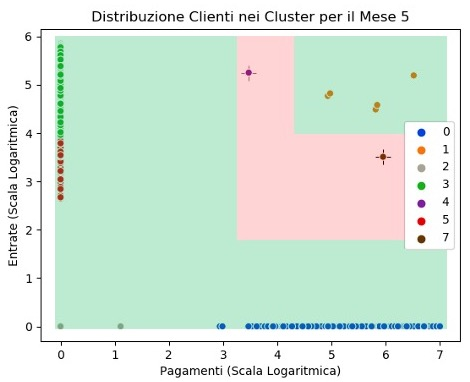
\includegraphics[width=0.7\textwidth]{M5.jpeg}
    \centering
    \caption{Distribuzione dei Clienti per il Mese 5}
    \label{fig:kaggle}
\end{figure}

\noindent L'albero estratto dal \textit{Decision Tree Classifier} viene riportato di seguito in cui vengono segnalate tramite \verb{class:1{ le foglie dove sono situate le anomalie, che corrispondo alle due anomalie visibili nella figura \ref{fig:kaggle}. \\

\begin{center}
\begin{minipage}{6cm}
\begin{Verbatim}[t][fontsize=\small, frame=single]
|--- PAGAMENTI <= 3.47
| |--- class: 0
|--- PAGAMENTI > 3.47
| |--- ENTRATE <= 1.75
| | |--- class: 0
| |--- ENTRATE > 1.75
| | |--- PAGAMENTI <= 4.20
| | | |--- class: 1
| | |--- PAGAMENTI > 4.20
| | | |--- ENTRATE <= 4.00
| | | | |--- class: 1
| | | |--- ENTRATE > 4.00
| | | | |--- class: 0
\end{Verbatim}
\end{minipage}
\end{center}
%\clearpage
\newpage

\noindent Le regole ottenute dal \textit{Decision Tree Classifier} per tutti i cluster del mese vengono di seguito riportate in notazione logaritmica e  in scala reale: \\
\vspace{1cm}

\begin{minipage}{7cm}
\raggedright
\begin{Verbatim}[t][fontsize=\small, frame=single]
Rule 1
Rule: PAGAMENTI <= 2953.173

Rule 3
Rule: PAGAMENTI > 2953.173
Rule: ENTRATE <= 56.877

Rule 5
Rule: PAGAMENTI > 2953.173
Rule: ENTRATE > 56.877
Rule: PAGAMENTI <= 15953.775
\end{Verbatim}
\end{minipage}%
\begin{minipage}{6cm}
\raggedleft
\begin{Verbatim}[t][fontsize=\small, frame=single]
Rule 7
Rule: PAGAMENTI > 2953.173
Rule: ENTRATE > 56.877
Rule: PAGAMENTI > 15953.775
Rule: ENTRATE <= 10014.66

Rule 8
Rule: PAGAMENTI > 2953.173
Rule: ENTRATE > 56.877
Rule: PAGAMENTI > 15953.775
Rule: ENTRATE > 10014.66 
\end{Verbatim}
\end{minipage}%
 \\
\begin{center}
    Regole in scala reale
\end{center}

\vspace{1.3cm}
 
\begin{minipage}{7cm}
\raggedright
\begin{Verbatim}[t][fontsize=\small, frame=single]
Rule 1
Rule: PAGAMENTI <= 3.47

Rule 3
Rule: PAGAMENTI > 3.47
Rule: ENTRATE <= 1.755

Rule 5
Rule: PAGAMENTI > 3.47
Rule: ENTRATE > 1.755
Rule: PAGAMENTI <= 4.203
\end{Verbatim}
\end{minipage}%
\begin{minipage}{6cm}
\raggedleft
\begin{Verbatim}[t][fontsize=\small, frame=single]
Rule 7
Rule: PAGAMENTI > 3.47
Rule: ENTRATE > 1.755
Rule: PAGAMENTI > 4.203
Rule: ENTRATE <= 4.001

Rule 8
Rule: PAGAMENTI > 3.47
Rule: ENTRATE > 1.755
Rule: PAGAMENTI > 4.203
Rule: ENTRATE > 4.001
\end{Verbatim}
\end{minipage}%
 \\
\begin{center}
    \\     Regole in scala logaritmica base 10 \\
\end{center}

\newpage
\noindent Confrontando le regole precedentemente estratte con l'albero ottenuto è possibile identificare nelle regole 5 e 7 le anomalie riscontrate in figura \ref{fig:kaggle}. Queste, riportate sia in notazione logaritmica (nella colonna di sinistra) in base dieci sia in scala reale (nella colonna di destra), verranno fornite all'operatore come spiegazione del comportamento utente nel mese corrente, nel caso specifico il quinto mese della challenge Kaggle.
\vspace{1cm}


\begin{minipage}{7cm}
\raggedright
\begin{Verbatim}[t][fontsize=\small, frame=single]
Rule 5
Rule: PAGAMENTI > 3.47
Rule: ENTRATE > 1.755
Rule: PAGAMENTI <= 4.203
\end{Verbatim}
\end{minipage}%
\begin{minipage}{6cm}
\raggedleft
\begin{Verbatim}[t][fontsize=\small, frame=single]
Rule 5
Rule: PAGAMENTI > 2953.173
Rule: ENTRATE > 56.877
Rule: PAGAMENTI <= 15953.775
\end{Verbatim}
\end{minipage}
\vspace{1cm}


\begin{minipage}{7cm}
\raggedright
\begin{Verbatim}[t][fontsize=\small, frame=single]
Rule 7
Rule: PAGAMENTI > 3.47
Rule: ENTRATE > 1.755
Rule: PAGAMENTI > 4.203
Rule: ENTRATE <= 4.001
\end{Verbatim}
\end{minipage}%
\begin{minipage}{6cm}
\raggedleft
\begin{Verbatim}[t][fontsize=\small, frame=single]
Rule 7
Rule: PAGAMENTI > 2953.173
Rule: ENTRATE > 56.877
Rule: PAGAMENTI > 15953.775
Rule: ENTRATE <= 10014.66
\end{Verbatim}
\end{minipage}




\section{Risultati su dati reali}

I risultati ottenuti utilizzando i dati della challenge Kaggle evidenziano come l'approccio proposto riesca ad isolare persone con comportamenti anomali e faciliti l'estrazione  di regole per descriverne il comportamento.

Avendo inoltre a disposizione una piccola parte di un dataset reale di una banca l'approccio è stato testato su questi ulteriori dati per capire i risultati ottenibili in un contesto sconosciuto. Il mese che prendiamo come riferimento è il mese 6 (Giugno) del 2018, dove sono presenti cinque utenti. Essi sono divisi in clienti (User, U) e aziende (Aziende, A) e dalla Figura \ref{fig:challenge} si può notare, che a fronte dei due cluster presenti nel mese, \verb{A1{ forma un cluster formato solo da se stesso che verrà quindi segnalato come anomalo.

Dal momento che il dataset presenta una numerosità molto ridotta le regole vengono generate su una sola metrica perché sufficiente a spiegare il comportamento dell'utente, in questo caso la metrica  è \verb{Min_amount{.

\begin{figure}[H]
    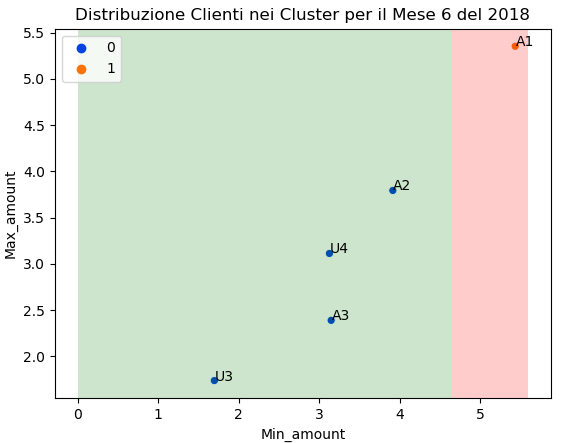
\includegraphics[width=0.8\textwidth]{6_2018.png}
    \centering
    \caption{Distribuzione dei Clienti per il Mese 6 del 2018}
    \label{fig:challenge}
\end{figure}

\noindent Il \textit{Decision Tree Classifier} a cui viene dato come input l'intero dataset del $6/2018$ produce il seguente albero con le seguenti regole riportate in scala reale (sinistra) e in scala logaritmica (destra). 
\vspace{0.2cm}

\begin{center}
\begin{minipage}{5cm}
\begin{Verbatim}[t][fontsize=\small, frame=single]
|--- Min_amount <= 4.64
|   |--- class: 0
|--- Min_amount >  4.64
|   |--- class: 1
\end{Verbatim}
\end{minipage}
\end{center}
\vspace{0.5cm}
\begin{minipage}{8cm}
\raggedright
\begin{Verbatim}[t][fontsize=\small, frame=single]
Rule 1
Rule: Min_amount <= 43294.397
Rule 2
Rule: Min_amount > 43294.397
\end{Verbatim}
\end{minipage}%
\begin{minipage}{6cm}
\raggedleft
\begin{Verbatim}[t][fontsize=\small, frame=single]
Rule 1
Rule: Min_amount <= 4.636
Rule 2
Rule: Min_amount > 4.636
\end{Verbatim}
\end{minipage}

\vspace{0.9cm}

\noindent Dai dati ricavati è possibile identificare nella regola $2$ l'anomalia che è possibile visualizzare nella figura \ref{fig:challenge}, essa si verifica quando \verb{Min_amount > 4.64{ (scala logaritmica in base dieci) oppure \verb{Min_amount > 43294.397{ (scala reale).

\noindent Dopo aver completato la ricerca di eventuali anomalie statiche per ogni mese del piccolo dataset reale, avendo a disposizione un arco temporale di diversi mesi, è stata condotta una breve analisi dinamica dei dati raccolti. 

Sono state quindi analizzate il numero di volte in cui un utente effettuava un cambio di cluster e le segnalazioni di anomalia nei mesi considerati. I cluster di appartenenza di ogni cliente nell'arco temporale sono riportati nella tabella \ref{tab:dinamiche}, dove il numero di cluster parte da $0$ fino ad un massimo di $2$ (quindi massimo $3$ cluster all'interno di un mese) e nel caso in cui non venga riportato nessun cluster il cliente in quel mese non ha effettuato transazioni.

\begin{table}[ht]
\centering
\begin{tabular}{|r||c|c|c|c|c|c|c|c|} \hline
Label & $1/2018$ & $2/2018$& $3/2018$ & $4/2018$ & $5/2018$ & $6/2017$ &$7/2018$ &$8/2018$\\ \hline
A1 & 0 & 0 & 0 & 2 & 0 & 1& 1 & 1 \\ \hline
U1 &  &  & 0   &   &   &  &   & \\ \hline
U2 &  &  & 0   &   &   &  &   & \\ \hline
A2 & 1 & 0 & 1 & 0 & 0 & 0& 0 &1 \\ \hline
U3 & 0 & 0 & 0 & 0 & 0 & 0& 0&0\\ \hline
A3 & 0 & 1 & 0 & 1 & 0 & 0& 1 &1\\ \hline
U4 & 0 & 0 & 0 & 0 & 1 & 0& 1&0\\ \hline
\end{tabular}
\caption{Composizione mensile dei cluster}
\label{tab:dinamiche}
\end{table}

\noindent Nella tabella \ref{tab:dinamiche} sopra riportata è possibile analizzare varie casistiche di distribuzione dei cluster, ad esempio andando a considerare l'utente \verb{U3{ è possibile notare come rimanga costante la sua presenza nel cluster $0$ e non effettui mai salti di cluster.  Un cliente che è possibile notare particolarmente anomalo è\verb{ A3 {che effettua numerosi cambiamenti di cluster e si posiziona come anomalo in cinque mesi su otto. Durante il mese $7/2018$ non viene considerato anomalo in quanto si muove con l'utente\verb{ U4{ con cui forma una sotto popolazione che parte dal cluster 0 per spostarsi nel 1. 

 Vengono segnalate come anomalie statiche rispettivamente:  il cliente\verb{ A2 {per il mese $1/2018$, il cliente\verb{ A3 {per il mese $2/2018$, il cliente\verb{ A2 {per il mese $3/2018$, il cliente\verb{ A1 {e \verb{A3{ per il mese $4/2018$, il cliente\verb{ U4 {per il mese $5/2018$ e il cliente\verb{ A1 {per il mese $6/2018$. 

Inoltre, è possibile notare che all'interno di uno stesso mese ($8/2018$) possono esserci più cluster ma nessuna anomalia di tipo statico, ed allo stesso tempo presentare un anomalia di tipo dinamico con il mese precedente ($7/2018$) anch'esso privo di anomalie statiche.

\section{Considerazioni}

Analizzando i risultati ottenuti applicando l'approccio proposto nel Capitolo $4$ al dataset della challenge Kaggle e al piccolo dataset reale possiamo vedere che è sempre possibile identificare utenti anomali all'interno di un mese o un periodo di tempo, nel caso in cui essi siano presenti. Infatti, in entrambi i dataset vengono trovate varie anomalie, con la differenza che nella challenge avendo un numero estremamente superiore di clienti si è potuto riscontrare un numero superiore di cluster e di utenti anomali.

La numerosità del campione considerato va inoltre ad influire sulla generazione delle regole per le anomalie. Per questo motivo, nel caso dei risultati provenienti dal dataset reale a seguito dell'applicazione del \textit{Decision Tree Classifier} risultava sufficiente esprimere la regola in funzione di un solo attributo, questo non accade invece nell'esempio riportato per la challenge dove risulta necessario l'impiego di due metriche per poter dare una spiegazione completa delle anomalie. 

 I soli risultati ottenuti dall'analisi focalizzata su un solo mese non sono però sufficienti a determinare su un utente sia effettivamente fraudolento. Per questo motivo è necessario implementare parallelamente a questa analisi un'analisi longitudinale su un lasso di tempo più o meno breve per investigare cosa quel utente abbia fatto nei mesi precedenti e successivi a quello considerato. 

%Approfondendo il suo comportamento e tracciandone un profilo che spieghi i suoi posizionamenti anomali nel periodo considerato, per ottenere dei dati più precisi che permettano di distinguere tra un comportamento plausibile ed uno sospetto. 
Non è sufficiente un singolo posizionamento anomalo o un singolo salto di cluster per avere la certezza di aver identificato un utente fraudolento, perché questi comportamenti posso essere facilmente influenzabili da agenti esterni (come festività o periodo fiscali) e non essere indice di attività malevola.

Eseguire quindi un analisi che comprenda sia un analisi statica che una dinamica porta ad avere un analisi discretamente completa del comportamento di un utente nel periodo considerato. In modo tale che, nel momento in cui tali analisi e segnalazioni pervengano all'operatore designato di analizzarle, esso possa eseguire il compito nel modo più corretto possibile avendo lui a disposizione tutti i dati necessari.

























\chapter{Conclusioni}
L'analisi condotta nel progetto di stage fornisce dei risultati promettenti per l'individuazione di potenziali clienti fraudolenti attraverso tecniche di Machine Learning, in particolare tramite l'impiego di algoritmi di clustering (Machine Learning non supervisionato) e alberi di decisione (Machine Learning supervisionato). 

I risultati evidenziano come sia sempre possibile suddividere, per ogni periodo di tempo desiderato, l'insieme degli utenti di una banca in cluster e analizzarne ogni composizione. In particolare, analizzandone la composizione è possibile identificare i cluster anomali per segnalarli al termine dell'analisi.
L'estrazione delle regole per ogni anomalia statica, che viene effettuata al termine della loro identificazione, può in un secondo momento essere impiegata come enciclopedia di schemi conosciuti di riciclaggio di denaro.

Queste informazioni possono diventare fondamentali per poter rilevare frodi o segnalare un comportamento potenzialmente fraudolento  in maniera tempestiva, permettendo quindi durante l'analisi di non rilevare solamente le attuali frodi ma prevenirne di future.


Inoltre, risulta di grande rilevanza l'analisi longitudinale dei vari mesi, unico strumento per poter eventualmente rilevare delle anomalie dinamiche di salto tra cluster, anche con utenti che staticamente non si configurano mai come anomali. Un cliente potrebbe non avere in nessun caso un comportamento che lo porti a discostarsi da uno dei cluster presenti nel mese, non posizionandosi mai come anomalia non verrebbe mai segnalato come tale e passerebbe sempre come utente non fraudolento. Implementando però l'analisi longitudinale è possibile investigare tutti quei clienti che, pur rimanendo sempre all'interno di un cluster, effettuano molti salti di cluster non giustificabili da un cambio di abitudini finanziarie (ad esempio un nuovo lavoro), riuscendo quindi ad identificarli e porli sotto osservazione. \\

\noindent L'analisi finale viene lasciata ad un operatore, a cui vengono forniti tutti i risultati ottenuti dall'analisi statica e dinamica dei mesi dell'orizzonte temporale considerato. L'operatore avrà il compito di controllare i clienti segnalati e le transazioni sospette per determinare l'effettiva presenza di una frode oppure rilevare un comportamento anomalo ma influenzato da agenti esterni e quindi perfettamente spiegabile.\\





\bibliographystyle{unsrtnat}
\bibliography{bibliografia}

\chapter*{Ringraziamenti}
La persona fondamentale senza la quale tutto questo non sarebbe stato possibile ed è quindi super importante ringraziare è ME STESSA \verb{(^U^){. Brava Artemisia, hai dato di matto un numero dignitoso di volte, ma avresti potuto fare di peggio, sono fiera di te!
\begin{center}
\begin{verbatim}
     ------------------ O==[]::::::::::::::::> ------------------
\end{verbatim}
\end{center}
\noindent Ed ora tutti gli altri... \\
Ringrazio il caffè che mi ha sostenuto durante tutto il percorso e la luna che mi guardava mentre scrivevo questa tesi, poche righe hanno avuto il privilegio di essere scritte alla luce del sole.

\noindent Ringrazio i miei bimbi ovvero tutto il Reparto Idra, la Nutoka e la Compagnia Mizar che mi hanno dato i sorrisi più belli e le soddisfazioni più grandi, ma anche taaaanti pensieri. 

\noindent Al dottorando, Riccardo, Ricky e la sua pazienza di non mandarmi al diavolo durante il tirocinio, soprattutto per le risposte ad ore imprecisate della sera e per la sua guida fondamentale per scoprire le magie di \textit{Python}, grazie.

\noindent Grazie al mio babbo che mi sostiene anche se a distanza. 


\noindent Ringrazio in ultimo (ma non per importanza) tutta quella banda di gente matta del dodicesimo ed anche gli infiltrati dagli altri piani, quindi: Francesco, Mattia, Sara, Erika, Daniel, Andrea, Martina e Vittorio (tutti in ordine puramente causale), grazie. \\


\noindent Di sicuro mi sarò scordata qualcuno e dovrà aspettare la tesi magistrale (sempre che ci arrivi).




\cleardoublepage
\thispagestyle{empty}
\vspace*{\stretch{1}}
\begin{flushright}
\itshape
\begin{tabular}{@{}l@{}}
E quindi uscimmo a riveder le stelle \\
\end{tabular}\\[3pt]
Dante Alighieri

\end{flushright}
\vspace{\stretch{2}}
\cleardoublepage
\end{document}



